\documentclass[12pt]{beamer}

\usepackage[brazil]{babel}
\usepackage[utf8]{inputenc}
\usepackage[T1]{fontenc}
\usepackage{animate}
\usepackage{amsbsy}
\usepackage{amsfonts}
\usepackage{amsmath}
\usepackage{amssymb}
\usepackage{amsthm}
\usepackage[toc,page,title,titletoc]{appendix}
\usepackage{dsfont}
\usepackage{esvect}
\usepackage[labelfont=bf]{caption}
\usepackage{subcaption}
\usepackage{float}
\usepackage[Glenn]{fncychap}%Sonny %Conny %Lenny %Glenn %Renje %Bjarne %Bjornstrup
\usepackage{graphicx}
\usepackage{indentfirst}%Para indentar os paragrafos automáticamente
\usepackage{lipsum}
\usepackage{longtable}
\usepackage{mathtools}
\usepackage{listings}%Inserir codigo do R no latex
\usepackage{multirow}
\usepackage{multicol}
\usepackage{csquotes}
\usepackage[maxcitenames=2,terseinits=true,natbib=true, style=authoryear, maxbibnames=99]{biblatex}
\addbibresource{../Referencias/Referencias.bib}
\usepackage[figuresright]{rotating}
\usepackage{spalign}
\usepackage{pgfplots}
\pgfplotsset{compat=1.17}
\usepackage{tikz}
\usepackage{color, colortbl}
\usepackage{url}
\usepackage{ragged2e}%para justificar o texto dentro de algum ambiente
\definecolor{Gray}{gray}{0.9}
\definecolor{LightCyan}{rgb}{0.88,1,1}


\usepackage[all]{xy}
\usepackage{hyperref,bookmark}
\hypersetup{
	colorlinks=true,
	linkcolor=blue,
	citecolor=red,
	filecolor=blue,
	urlcolor=blue,
}

%\usetheme{Madrid}
%\usecolortheme[RGB={193,0,0}]{structure}
\usetheme{metropolis}
\definecolor{mycolor}{RGB}{34, 45, 50}
\setbeamercolor{structure}{fg=mycolor}
%\usepackage{mathpazo} % Fonte elegante para matemática
\usepackage{helvet} % Fonte sans-serif para texto
\renewcommand{\familydefault}{\sfdefault} % Definir fonte padrão como sans-serif
%\setbeamertemplate{footline}[frame number]
%\setbeamertemplate{footline}[text line]{%
%  \parbox{\linewidth}{\vspace*{-8pt}\hfill\date{}\hfill\insertshortauthor\hfill\insertpagenumber}}
\beamertemplatenavigationsymbolsempty
\renewcommand{\vec}[1]{\mbox{\boldmath$#1$}}
\newtheorem{Teorema}{Teorema}
\newtheorem{Proposicao}{Proposição}
\newtheorem{Definicao}{Definição}
\newtheorem{Corolario}{Corolário}
\newtheorem{Demonstracao}{Demonstração}
\newcommand{\bx}{\ensuremath{\bar{x}}}
\newcommand{\Ho}{\ensuremath{H_{0}}}
\newcommand{\Hi}{\ensuremath{H_{1}}}
\newcounter{saveenumi}
\newcommand{\seti}{\setcounter{saveenumi}{\value{enumi}}}
\newcommand{\conti}{\setcounter{enumi}{\value{saveenumi}}}

\apptocmd{\frame}{}{\justifying}{} % Allow optional arguments after frame.

\title{Estatística I}
\author{Prof. Fernando de Souza Bastos \texorpdfstring{\\ fernando.bastos@ufv.br}{}}
\institute{Departamento de Estatística \texorpdfstring{\\ Universidade Federal de Viçosa}{}\texorpdfstring{\\ Campus UFV - Viçosa}{}}
\date{}
\newcommand\mytext{Aula 2}
\newcommand\mytextt{Fernando de Souza Bastos}
\newcommand\mytexttt{\url{https://ufvest.github.io/}}

\makeatletter
\setbeamertemplate{footline}
{
  \leavevmode%
  \hbox{%
  \begin{beamercolorbox}[wd=.3\paperwidth,ht=2.25ex,dp=1ex,center]{author in head/foot}%
    \usebeamerfont{author in head/foot}\mytext
  \end{beamercolorbox}%
  \begin{beamercolorbox}[wd=.3\paperwidth,ht=2.25ex,dp=1ex,center]{title in head/foot}%
    \usebeamerfont{title in head/foot}\mytextt
  \end{beamercolorbox}%
  \begin{beamercolorbox}[wd=.35\paperwidth,ht=2.25ex,dp=1ex,right]{site in head/foot}%
    \usebeamerfont{site in head/foot}\mytexttt\hspace*{2em}
    \insertframenumber{} / \inserttotalframenumber\hspace*{2ex} 
  \end{beamercolorbox}}%
  \vskip0pt%
}
\makeatother

\providecommand{\arcsin}{} \renewcommand{\arcsin}{\hspace{2pt}\textrm{arcsen}}
\providecommand{\sin}{} \renewcommand{\sin}{\hspace{2pt}\textrm{sen}}
%\newtheorem{Teorema}{Teorema}
%\newtheorem{Proposicao}{Proposição}
%\newtheorem{Definicao}{Definição}
%\newtheorem{Corolario}{Corolário}
%\newtheorem{Demonstracao}{Demonstração}

\titlegraphic{\hspace*{8cm}\href{https://fsbmat-ufv.github.io/}{
\includegraphics[width=2cm]{figs/mylogo.png}}
}

% Layout da pagina
\hypersetup{pdfpagelayout=SinglePage}
\begin{document}
%\SweaveOpts{concordance=TRUE}

\frame{\titlepage}

\begin{frame}{}
\frametitle{\bf Sumário}
\tableofcontents
\end{frame}

\section{Somatórios}
\begin{frame}{}
\frametitle{Somatório}
\begin{block}{}
\justifying
O somatório é uma forma abreviada para representação de somas. Podemos defini-lo como o operador matemático para a soma dos termos de uma sequência. Usualmente, um somatório é representado pela letra grega sigma maiúscula $(\sum)$ e é definido por:
\begin{equation}
{\displaystyle \sum_{i=m}^{n}x_{i}=x_{m}+x_{m+1}+\cdots+x_{n}.}
\end{equation}
em que $\{ x_{k} \}_{k\in \mathds{N}}$ é uma sequência dada, $i$ é o índice do somatório, $m$ denota o limite inferior e $n$ o limite superior.
\end{block}
\end{frame}

\begin{frame}{}
\frametitle{Somatório}
\begin{block}{}
\justifying
Como exemplo note que
\begin{equation}
{\displaystyle \sum_{i=1}^{n}i=1+2+3+\cdots+(n-2)+(n-1)+n}
\end{equation}
Se lê: ``Soma de $i,$ para $i=1$ até $n.$''
\end{block}
\pause
\begin{block}{}
\justifying
ou,
\begin{equation}
{\displaystyle \sum_{i=0}^{k}(2i+1)=1+3+\cdots+(2k-1)+(2k+1)}
\end{equation}
que se lê: ``Soma de $(2i+1),$ para $i=0$ até $k.$''
\end{block}
\end{frame}

\begin{frame}{}
\frametitle{Propriedades}
\begin{block}{}
\justifying
\begin{enumerate}
\item ${\displaystyle \sum_{i=m}^{n}ax_{i}=a\sum_{i=m}^{n}x_{i}\ \forall a\in \mathds{R}, m,n\in \mathds{Z}.}$
\item ${\displaystyle \sum_{i=m}^{n}K=[(n-m)+1]K},$ $K$ constante real qualquer. Em particular para $m=1,$ temos 
${\displaystyle \sum_{i=1}^{n}K=nK}.$
    \seti
\end{enumerate}
\end{block}
\end{frame}

\begin{frame}{}
\frametitle{Propriedades}
\begin{block}{}
\justifying
\begin{enumerate}
    \conti
\item ${\displaystyle \sum_{i=m}^{n}(a_{i}x_{i}+b_{i}z_{i})=\sum_{i=m}^{n}(a_{i}x_{i})+
\sum_{i=m}^{n}(b_{i}z_{i}),\ \forall m,n\in \mathds{Z}.}$ 
\item ${\displaystyle \sum_{i=k}^{n}(x_{i}-x_{i+1})=x_{k}-x_{n+1}}$  
\item ${\displaystyle \sum_{k=0}^{n}K=\sum_{k=1}^{n}K=\dfrac{n(n+1)}{2}}$ (Soma de Gauss) 
    \seti
\end{enumerate}
\end{block}
\end{frame}

\begin{frame}{}
\frametitle{Soma de Gauss}
\begin{block}{}
\begin{minipage}{0.4\textwidth}
\begin{figure}[H]
    \centering
\caption{Imagem retirada do \citet{wikiGauss}. Visitado em 28/06/2021.}
    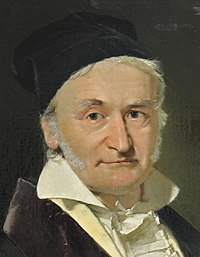
\includegraphics[width=0.8\textwidth]{figs/Gauss.jpg}
    %\label{figRotulo}
  \end{figure}
\end{minipage}\hfill
\begin{minipage}{0.6\textwidth}
%{\small Considere} ${\scriptstyle %S=1+2+3+\cdots+98+99+100}$
%\begin{align*}
%    1+100&=101\\
%    2+99&=101\\
%    3+98&=101\\
%\vdots \quad   &=\quad \vdots\\
%    49+52&=101\\
%    50+51&=101\\
%    50\times 101&=5050
%\end{align*}
Considere $S_{N}=a_{1}+a_{2}+\cdots + a_{n-1}+a_{n}.$ A fórmula abaixo foi obtida por Johann Carl Friedrich Gauss (``O principe da Matemática''). 
$$S_{N}=\dfrac{(a_{1}+a_{n})n}{2}$$
\end{minipage}
\end{block}
\end{frame}

\begin{frame}{}
\frametitle{Cuidado!}
\begin{block}{}
\justifying
\begin{enumerate}
\item ${\displaystyle \sum_{i=1}^{n}x_{i}y_{i}\neq\Big(\sum_{i=1}^{n}x_{i}\Big)\Big(\sum_{i=1}^{n}y_{i}\Big)}$\pause
\item ${\displaystyle \sum_{i=m}^{n}a(x_{i}+k)\neq\sum_{i=m}^{n}ax_{i}+k}$\pause
\item ${\displaystyle \sum_{i=1}^{n}a_{i}^{2}\neq \Biggl(\sum_{i=1}^{n}a_{i}\Biggl)^{2}}$ 
\end{enumerate}
\end{block}
\end{frame}

\begin{frame}{}
\frametitle{}
\begin{block}{}
\justifying
{\bf Soma infinita:} é a soma de infinitos termos, a qual, espera-se que convirja para um determinado
valor. É muito aplicada na teoria da probabilidade na definição de modelos em espaços infinitos discretos.
$${\displaystyle \sum_{i=1}^{\infty}x_{i}=x_{1}+x_{2}+\cdots}$$
\end{block}
\end{frame}

\begin{frame}{}
\frametitle{}
\begin{block}{}
\justifying
{\bf Exemplo:} Qual é a fração geradora da dizima $3.55555\cdots$?
\begin{align*}
3.55555\cdots &=3+0.5+0.05+0.005+0.0005+0.00005+\cdots\\
&=3+\dfrac{5}{10}+\dfrac{5}{100}+\dfrac{5}{1000}+\dfrac{5}{10000}+\cdots\\
&=3+{\displaystyle \sum_{i=1}^{\infty}\dfrac{5}{10^{i}}}\\
&=3+\dfrac{5/10}{1-1/10}\\
&=3+\dfrac{5}{9}=\dfrac{32}{9}
\end{align*}
\end{block}
\end{frame}

\section{Somatório Duplo}
\begin{frame}{}
\frametitle{Somatório Duplo}
\vspace{-0.5cm}
\begin{block}{}
\begin{table}[H]
    \centering
    \begin{tabular}{c|ccccccc}
          & $1$       &$2$        &$\ldots$& $j$       &$\ldots$& $s$       &\\
    \hline
        1 & $X_{11}$  & $X_{12}$  &$\ldots$& $X_{1j}$  &$\ldots$& $X_{1s}$  &${\displaystyle \sum_{j=1}^{s}X_{1j}}$  \\
        2 & $X_{21}$  & $X_{22}$  &$\ldots$& $X_{2j}$  &$\ldots$& $X_{2s}$  &${\displaystyle \sum_{j=1}^{s}X_{2j}}$  \\
    \ldots& $\ldots$  & $\ldots$  &$\ldots$& $\ldots$  &$\ldots$& $\ldots$  &$ \ldots$\\
        i & $X_{i1}$  & $X_{i2}$  &$\ldots$& $X_{3j}$  &$\ldots$& $X_{is}$  &${\displaystyle \sum_{j=1}^{s}X_{ij}}$  \\
    \ldots& $\ldots$  & $\ldots$  &$\ldots$& $\ldots$  &$\ldots$& $\ldots$  &$ \ldots$\\
        r & $X_{r1}$  & $X_{r2}$  &$\ldots$& $X_{rj}$  &$\ldots$& $X_{rs}$  &${\displaystyle \sum_{j=1}^{s}X_{rj}}$  \\
        \hline
          &${\displaystyle \sum_{i=1}^{r}X_{i1}}$ &${\displaystyle \sum_{i=1}^{r}X_{i2}}$&$\ldots$ &${\displaystyle \sum_{i=1}^{r}X_{ij}}$&$\ldots$ &${\displaystyle \sum_{i=1}^{r}X_{is}}$&$G$
    \end{tabular}
    \label{tab:my_label}
\end{table}
\end{block}
\end{frame}

\begin{frame}{}
\frametitle{Somatório Duplo}
\vspace{-0.3cm}
\begin{block}{}
$X_{ij}\rightarrow i=1,2,\cdots,r$ é o índice da linha\\
$X_{ij}\rightarrow j=1,2,\cdots,s$ é o índice da coluna\\
$G$ é o total geral:
\begin{align*}
G=&{\displaystyle \sum_{i=1}^{r}X_{i1}
                +\sum_{i=1}^{r}X_{i2}
                +\cdots
                +\sum_{i=1}^{r}X_{ij}
                +\cdots
                +\sum_{i=1}^{r}X_{is}}\\
=&{\displaystyle \sum_{i=1}^{r}(X_{i1}
                + X_{i2}
                +\cdots
                + X_{ij}
                +\cdots
                + X_{is}})\\
=&{\displaystyle \sum_{i=1}^{r}\sum_{j=1}^{s}X_{ij}}\\
=&{\displaystyle \sum_{i=1,j=1}^{r,s}X_{ij}}\\
=&X_{\cdot \cdot}
\end{align*}
\end{block}
\end{frame}

\begin{frame}{}
\frametitle{Somatório Duplo}
\begin{block}{}
\begin{center}
    Total da i-ésima linha: ${\displaystyle \sum_{j=1}^{s}}X_{ij}=X_{i\cdot}$\\
    Total da j-ésima coluna: ${\displaystyle \sum_{i=1}^{r}}X_{ij}=X_{\cdot j}$
\end{center}
\end{block}
\end{frame}

\section{Produtório}
\begin{frame}{}
\frametitle{Produtório}
\begin{block}{}
\justifying
De forma alternativa, como na adição, o produto pode ser escrito usando-se um símbolo de produto, chamado 
produtório $\prod$ que é a letra pi maíuscula no alfabeto grego.
$${\displaystyle \prod_{i=1}^{n}x_{i}=x_{1}x_{2}\cdots x_{n}}$$
\end{block}
\nocite{Morettin09, Apostila, eric, montgomery2016, Bastos2025}
\end{frame}

\begin{frame}[allowframebreaks]
\frametitle{}
\printbibliography
\end{frame}

\end{document} 
